
\chapter{Formal Concept Analysis}
\label{cha:form-conc-analys}

\todo[inline]{Write: introductory text, some historical notes, some subfield classification}

\section{Formal Contexts and Concept Lattices}
\label{sec:form-cont-cont}

We introduce the basic notions of formal concept analysis in this section.  Most
importantly, we shall discuss how formal concept analysis allows us to represent
complete lattices in terms of \emph{formal concept lattices} using the notion of
\emph{formal contexts}.  Moreover, we shall introduce the notion of a \emph{Galois
  connection} between two ordered sets.

Let us briefly repeat the basic notions of order theory which are relevant for our further
considerations.  Let $P$ be a set and let ${\le} \subseteq P \times P$ be a binary
relation on $P$.  Then the pair $(P, \le)$ is called an \emph{(partially) ordered set} if
$\le$ is reflexive, transitive and antisymmetric.  Such structures can be visualize in
terms of \emph{order diagrams} (often called \emph{Hasse diagrams}) if they are finite
(and not too large).  For this way call two elements $x, y \in P$ with $x < y$
\emph{directly neighbored} in $(P, \le)$ if and only if there does not exist an element $z
\in P$ such that $x < z < y$.  Then to visualize $(P, \le)$ we mark for every element
$x \in P$ a node $v_x$ on the plane such that whenever $x < y$ it is true that the
ordinate (the second coordinate) of $v_x$ is strictly smaller then the one of $v_y$.
Then, we draw for every two elements $x, y$ with $x < y$ which are directly neighbored in
$(P, \le)$ an undirected line from $v_x$ to $v_y$.

Observe that this construction is not unique, and are many different possibilities (good
and bad) to visualize ordered sets in this way.  Also note that the naming $v_x$ of
vertices for elements $x$ is arbitrary and can be chosen as it suits.

\begin{Example}
  \label{expl:1}
  Let us consider the set $\set{1, 2, 3}$ with the usual order $\le$ on natural numbers.
  Then a line diagram of this order set is
  \begin{center}
    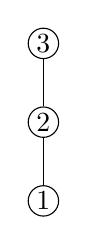
\begin{tikzpicture}[every node/.style = {draw, circle, inner sep = 1pt}]
      \node (A) {$3$};
      \node[below of=A] (B) {$2$};
      \node[below of=B] (C) {$1$};
      \draw (A) -- (B);
      \draw (B) -- (C);
    \end{tikzpicture}
  \end{center}
  We can readily read of this diagram that $1 < 2$ and $2 < 3$, because there are lines
  connecting the corresponding vertices.  But we can also see that $1 < 3$ because there
  is an \emph{ascending path} from $1$ to $3$.
\end{Example}

More generally, in a line diagram of an ordered set $(P, \le)$, two elements $x, y \in P$
satisfy $x \le y$ if and only if there is an ascending path from $x$ to $y$ in the line
diagram (where also paths of length 0 are allowed).

\begin{Example}
  \label{expl:2}
  Let $P = \set{ 1, 2, 3 }$ and consider the ordered set $(\subsets{\set{1,2,3}},
  \subseteq)$, where $\subsets{\set{1,2,3}}$ denotes the set of all subsets of
  $\set{1,2,3}$.  This set can be visualized as a line diagram as follows:
  \begin{center}
    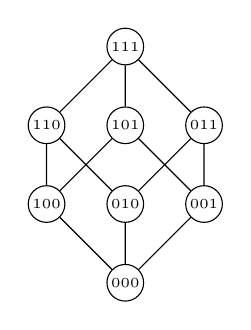
\begin{tikzpicture}[every node/.style = {draw, circle, inner sep = 1pt}]
      \node (0) at (0,0)  {\tiny 000};
      \node (1) at (-1,1) {\tiny 100};
      \node (2) at (0, 1) {\tiny 010};
      \node (3) at (1, 1) {\tiny 001};
      \node (4) at (-1,2) {\tiny 110};
      \node (5) at (0,2)  {\tiny 101};
      \node (6) at (1,2)  {\tiny 011};
      \node (7) at (0,3)  {\tiny 111};
      \draw{
        (0) -- (1)
        (0) -- (2)
        (0) -- (3)
        (1) -- (4)
        (1) -- (5)
        (2) -- (4)
        (2) -- (6)
        (3) -- (5)
        (3) -- (6)
        (4) -- (7)
        (5) -- (7)
        (6) -- (7)
      };
    \end{tikzpicture}
  \end{center}
  Here we denote subsets of $\set{1,2,3}$ by sequences of 0 and 1, meaning that if the
  first position is 1 if and only if the number 1 is an element of the corresponding
  subset, and so on.  Then 101 corresponds to the set $\set{1,3}$.
\end{Example}

An element $x \in P$ is said to be the \emph{smallest element} of $(P, \le)$ if and only
if $x \le y$ is true for all $y \in P$.  Likewise, $x$ is the \emph{greatest element} of
$(P, \le)$ if and only if $y \le x$ is true for all $y \in P$.  Note that neither smallest
nor greatest elements have to exist in $P$.  However, if these elements exist, they are
unique up to equivalence.

Let $Q \subseteq P$.  An element $x \in Q$ is said to be the \emph{smallest element} in
$Q$ (with respect to $(P, \le)$) if and only if $x \le y$ is true for all $y \in Q$;
\emph{greatest element} in $Q$ are defined likewise.  Again, neither smallest nor greatest
elements in $Q$ have to exist.

Let $x \in P$.  The \emph{order-ideal} ${\downarrow}x$ and the \emph{order-filter}
${\uparrow} x$ of $x$ in $(P, \le)$ are defined as
\begin{align*}
  {\downarrow} x &:= \set{ y \in P \mid y \le x },\\
  {\uparrow} x &:= \set{ y \in P \mid x \le y }.
\end{align*}
In other words, ${\downarrow} x$ contains all elements which are \emph{below} $x$ in $(P,
\le)$, and ${\uparrow} x$ contains all elements which are \emph{above} $x$ in $(P, \le)$.

Let again $Q \subseteq P$.  Then the sets ${\downarrow} Q$ and ${\uparrow} Q$ defined as
\begin{align*}
  {\uparrow} Q &:= \bigcap_{q \in Q} {\uparrow} q,\\
  {\downarrow} Q &:= \bigcap_{q \in Q} {\downarrow} q
\end{align*}
are called the set of \emph{upper bounds} and \emph{lower bounds} of $Q$ in $(P, \le)$,
respectively, where we employ the convention that $\bigcap \emptyset = P$.  If ${\uparrow}
Q$ has a smallest element (a \emph{least upper bound}) in $(P, \le)$, it is called the
\emph{supremum} of $Q$ in $(P, \le)$ and is denoted by $\sup Q$.  Likewise, if
${\downarrow} Q$ has a greatest element (a \emph{greatest lower bound}) in $(P, \le)$,
then it is called the \emph{infimum} of $Q$ in $(P, \le)$ and is denoted by $\inf Q$.

Note again that neither infimum nor supremum have to exist in $(P, \le)$.

\begin{Example}
  \label{expl:3}
  Let $P = \set{ a, b, c }$ and let $\le$ be given by the smallest order relation that
  satisfies $a < b$ and $a < c$.  Then $\inf\set{b,c}$ exists in $(P, \le)$ and is equal
  to $a$.  However, $\sup\set{b, c}$ does not exist in $(P, \le)$, as ${\uparrow} b \cap
  {\uparrow} c = \emptyset$.
\end{Example}

\noindent%
Structures in which supremum and infimum always exist for \emph{finite} sets $Q$ are
called \emph{lattices}.  If the sets $Q$ can be chosen arbitrary, then we call such a
structure a \emph{complete lattice}.

\begin{Definition}[Lattice]
  \label{def:lattice}
  Let $\alg L = (L, \le)$ be an ordered set.  Then $\alg L$ is called a \emph{lattice} if
  and only if for each finite $Q \subseteq L$ there exist both $\sup Q$ and $\inf Q$ in
  $\alg L$.  If for all $Q \subseteq L$ there exist both $\sup Q$ and $\inf Q$ in $\alg
  L$, then $\alg L$ is called a \emph{complete lattice}.
\end{Definition}

\noindent%
Note that every finite lattice is also a complete lattice.  Moreover, every complete
lattice has a smallest and greatest element, given by $\sup\emptyset$ and $\inf\emptyset$,
respectively.  Furthermore, every ordered set $(P, \le)$ in which the supremum exists for
each $Q \subseteq P$ is already a complete lattice, as the infimum is then given by
\begin{equation*}
  \inf Q = \sup\set{ x \in P \mid \forall y \in Q \holds x \le y }.
\end{equation*}
The same is of course true if supremum and infimum are exchanged.

The ordered sets from Examples~\ref{expl:1} and~\ref{expl:2} are lattices, but not the one
from~\ref{expl:3}.  More generally, if $P$ is a set, then $(\subsets{P}, \subseteq)$ is
always a complete lattice.

The study of lattices as mathematical structures has received much interest over the last
decades and thus constitutes a major branch of order theory.\todo{cite main book on
  lattice theory} However, (complete) lattices also allow for a quite natural
interpretation as a hierarchy of \emph{generalizations} and \emph{specializations}: an
element $x$ is below an element $y$ if and only if $x$ is more \emph{special} than $y$, or
alternatively, if $y$ is more \emph{general} than $x$.  Then for a set $Q$ of elements its
supremum $\sup Q$ can be thought of as a \emph{most-specific generalization} of all
elements in $Q$, and $\inf Q$ can be seen likewise as the most \emph{general
  specialization} of all elements in $Q$.

Formal concept analysis now provides an approach to understand complete lattice in terms
of this interpretation, by representing these lattices in terms of \emph{objects} and
their \emph{attributes}.  For this, we need to introduce the notion of a \emph{formal
  context}.

\begin{Definition}[Formal Context]
  \label{def:formal-context}
  A \emph{formal context} $\con K$ is constituted of three sets $G, M, I$, where $I
  \subseteq G \times M$.  Most often, we shall identify $\con K$ with the triple $(G, M,
  I)$, \ie $\con K = (G, M, I)$.  We shall call $G$ the set of \emph{objects} of $\con K$,
  $M$ the set of \emph{attributes} of $\con K$ and $I$ the \emph{incidence} of $\con K$.
  Two formal contexts are equal if and only if their sets of objects, attributes and their
  incidences are equal, respectively.
\end{Definition}

Formal contexts can be thought of as simple data structures which record for a set of
objects the set of attributes those objects have.  More precisely, we shall say that in a
formal context $\con K$ an object $g \in G$ \emph{has} an attribute $m$ if and only if
$(g, m) \in I$.

\begin{Example}
  \label{expl:star-trek}
  Let us consider a small toy example $\con K_{\mathsf{TNG}}$ to illustrate the definition
  of a formal context.  As sets of objects we choose some fictional characters from
  \emph{Star Trek: The Next Generation}, namely
  \begin{equation*}
    G := \set{ \mathsf{Picard}, \mathsf{Worf}, \mathsf{Data}, \mathsf{BorgQueen} }.
  \end{equation*}
  As sets of attributes we choose
  \begin{equation*}
    M := \set{ \mathsf{Human}, \mathsf{Honorable}, \mathsf{Artificial}, \mathsf{Star
        Fleet} }.
  \end{equation*}
  To illustrate the incidence relation of our examples formal context we make use of a
  \emph{cross table}, \ie we depict $\con K_{\mathsf{TNG}}$ as a table where the rows are
  labeled with objects and the columns are labeled with attributes.  Then in every cell we
  write a cross if and only if the objects labeling the corresponding row has the
  attribute labeling the corresponding column.
  \begin{equation*}
    \def\x{\times}
    \begin{array}{r|*{4}{c}}
      \toprule
      \con K_{\mathsf{TNG}} & \mathsf{Human} & \mathsf{Honorable} & \mathsf{Artificial} & \mathsf{Star Fleet} \\
      \midrule
      \mathsf{Picard} & \x & \x & & \x \\
      \mathsf{Worf} & & \x & & \x \\
      \mathsf{Data} & & \x & \x & \x \\
      \mathsf{BorgQueen} & & & \x & \\
      \bottomrule
    \end{array}
  \end{equation*}
  Then \textsf{BorgQueen} has the attribute \textsf{Artificial}, but not \textsf{Honorable}.
\end{Example}

To now expose the connection between formal contexts on the one hand and complete lattices
on the other we shall introduce the \emph{derivation operators} in formal contexts.

\begin{Definition}[Contextual Derivation]
  \label{def:contextual-derivation}
  Let $\con K = (G, M, I)$ be a formal context and let $A \subseteq G$ be a set of
  objects.  Then the set of \emph{common attributes} $A'$ of $A$ is defined to be
  \begin{equation*}
    A' := \set{ m \in M \mid \forall g \in G \holds (g, m) \in I }.
  \end{equation*}
  Likewise, for a set $B \subseteq M$ of attributes we define the set $B'$ of \emph{shared
    objects} as
  \begin{equation*}
    B' := \set{ g \in G \mid \forall m \in M \holds (g, m) \in I }.
  \end{equation*}
  The functions $A \mapsto A'$ and $B \mapsto B'$ are called the \emph{derivation
    operators} of $\con K$, and the sets $A'$ and $B'$ are called the \emph{derivations}
  of $A$ and $B$ in $\con K$, respectively.
\end{Definition}

For $(A')'$ we may also simply write $A''$.

Note that both derivation operators are denoted by $(\cdot)'$, which usually does not lead
to confusion, as it is most often clear from the context whether we deal with a set of
objects or a set of attributes from which we want to compute its derivation.  If it
nevertheless happens that a single name for the derivation operator leads to confusion,
then we shall locally introduce separate names for both of them.

What occurs more often, for example in Chapters~\ref{cha:expl-conf}
and~\ref{cha:model-expl-conf}, is the derivation of sets in \emph{different contexts}.
For example we may have given two formal contexts $\con K_1 = (G_1, M_1, I_1)$ and $\con
K_2 = (G_2, M_2, I_2)$ and a set $A \subseteq M_1 \cap M_2$.  Then when writing $A'$ it is
not clear in which context we do the derivation.  To remedy this, we shall add a subscript
to the set $A$ to make clear of which context we consider it as a set of attributes:
$A_{\con K_1}$ denotes the set $A$ considered as a set of attributes in $\con K_1$, and
likewise $A_{\con K_2}$.  While this notation is not useful as it stands, it becomes handy
if we consider derivations of $A$: $(A_{\con K_1})'$ denotes the derivation of $A$ in the
formal context $\con K_1$, while $(A_{\con K_2})'$ does the same for the formal context
$\con K_2$.  Of course, we can drop the parentheses if they do not lead to ambiguity and
write $A_{\con K_1}'$ and $A_{\con K_2}'$ instead.  Of course, the same can be done for
sets of objects.  In particular, instead of writing $(A_{\con K_1}')_{\con K_1}'$ we shall
often only write $A_{\con K_1}''$.

\begin{Example}
  \label{expl:4}
  Consider our Star Trek example context from~\ref{expl:star-trek} and let $A :=
  \set{\mathsf{Human}}$.  Then $A' = \set{ \mathsf{Picard} }$, $A'' = \set{
    \mathsf{Human}, \mathsf{Honorable}, \mathsf{Star Fleet} }$, and $A''' = \set{
    \mathsf{Picard} } = A'$.
\end{Example}

The case that $A''' = A'$ is true in the previous example is not a coincidence, but rather
an instance of a more general result: the derivation operators of a formal context form a
\emph{Galois connection} between the ordered sets $(\subsets{G}, \subseteq)$ and
$(\subsets{M}, \subseteq)$.

\begin{Lemma}
  \label{lem:derivation-is-galois-connection}
  Let $\con K = (G, M, I)$ be a formal context and let $A \subseteq M$ and $B \subseteq
  G$.  Then it is true that
  \begin{equation}
    \label{eq:1}
    A \subseteq B' \iff B \subseteq A'.
  \end{equation}
  From this the following properties of the derivation operators of $\con K$ can be
  derived: let $A, A_1, A_2 \subseteq M$ and $B, B_1, B_2 \subseteq G$.  Then
  \begin{enumerate}[i. ]
  \item $A_1 \subseteq A_2 \implies A_2' \subseteq A_1'$,
  \item $B_1 \subseteq B_2 \implies B_2' \subseteq B_1'$,
  \item $A \subseteq A''$,
  \item $B \subseteq B''$,
  \item $A' = A'''$,
  \item $B' = B'''$.
  \end{enumerate}
\end{Lemma}
%
In the proof of the lemma we shall only show Equation~\eqref{eq:1}, as the remaining
claims are a then an immediate consequence of the more general result
Lemma~\ref{lem:properties-of-galois-connections} on Galois connections.
%
\begin{Proof}[\thref{lem:derivation-is-galois-connection}]
  We can easily compute that
  \begin{align*}
    A \subseteq B'
    & \iff \forall m \in A \holds m \in B' \\
    & \iff \forall m \in A \;\forall g \in B \holds (g,m) \in I \\
    & \iff \forall g \in B \;\forall m \in A \holds (g,m) \in I \\
    & \iff \forall g \in B \holds g \in A' \\
    & \iff B \subseteq A'
  \end{align*}
  which shows the claim.
\end{Proof}

Another useful property of the derivation operators is
\begin{equation*}
  A' = \bigcap_{a \in A} \set{a}'
\end{equation*}
for $A \subseteq M$.  This can easily be generalized into the following statement.

\begin{Lemma}
  \label{lem:piecewise-derivation}
  Let $\con K = (G, M, I)$ be a formal context, let $A \subseteq M$ and let $(B_j \mid j
  \in J)$ be a family of sets $B_j \subseteq M$ such that
  \begin{equation*}
    A = \bigcup_{j \in J} B_j.
  \end{equation*}
  Then
  \begin{equation}
    \label{eq:2}
    A' = \bigcap \set{ B_j' \mid j \in J }.
  \end{equation}
  In particular, for every $\mathcal{A} \subseteq \subsets{M}$ it is true that
  \begin{equation}
    \label{eq:3}
    \bigcap_{A \in \mathcal{A}} A' = \bigl(\bigcup_{A \in \mathcal{A}} A'\bigr).
  \end{equation}
\end{Lemma}
%
Of course, the same is true if $A$ and all $B_j$ are sets of objects instead of sets of
attributes.
%
\begin{Proof}[\thref{lem:piecewise-derivation}]
  Since $B_j \subseteq A$ for all $j \in J$, we can infer from
  \thref{lem:derivation-is-galois-connection} that $A' \subseteq B_j'$.  It therefore
  suffices to show that $A' \supseteq \bigcap \set{ B_j' \mid j \in J }$.

  To this end, let $g \in \bigcap \set{ B_j' \mid j \in J }$.  Then $g \in B_j'$ for each
  $j \in J$, and therefore $\set{g}' \supseteq B_j$, again for all $j \in J$.  Since $A =
  \bigcup_{j \in J} B_j$, we obtain from this that $\set{g}' \supseteq A$, and thus $g \in
  A'$, as required.
\end{Proof}

We have claimed earlier that there exists a close connection between complete lattices on
the one hand and formal contexts on the other.  Having introduced the derivation
operators, we are now able to expose this connection.  To this end, we shall introduce the
notion of \emph{formal concepts} of a formal context.

\begin{Definition}[Formal Concept]
  \label{def:formal-concept}
  Let $\con K = (G, M, I)$ be a formal context.  Then a \emph{formal concept} of $\con K$
  is a pair $(A, B)$ such that $A \subseteq G, B \subseteq M$, and $A' = B, B' = A$ holds.
  The first entry of a formal concept is called its \emph{extent}, and the second one
  called its \emph{intent}.  The set of all formal concepts of $\con K$ is denoted by
  $\BV(\con K)$, the set of all extents of (formal concepts of) $\con K$ is denoted by
  $\Ext\con K$, and the set of all intents of (formal concepts of) $\con K$ is denoted by
  $\Int\con K$.
\end{Definition}

Note that for each $A \subseteq M$, the pair $(A, A')$ is a formal concept of $\con K$.
Moreover, a set $A \subseteq M$ is an intent of $\con K$ if and only if $A = A''$: if $A =
A''$, then $(A'', A')$ is a formal concept of $\con K$, and if $(A, B)$ is a formal
concept of $\con K$, then $A'' = B' = A$.  The same is of course true for $B \subseteq G$:
$B$ is an extent of $\con K$ if and only if $B = B''$.

Formal concepts have a strong philosophical motivation, as they are an attempt to
formalize the rather vague notion of a \emph{concept}.  This formalization is based on the
perception that every formal concept is uniquely determined by the objects which are
instances of it, its \emph{extension}, as well as by a characterization in terms of
attributes, its \emph{intension}.  We shall, however, not pursue this philosophical
motivation any further here, as it is not immediately relevant for our work.
See~\cite{fca-book} for further discussion and references.

\begin{Example}
  \label{expl:5}
  Two formal concepts of $\con K_{\mathsf{TNG}}$ from Example~\ref{expl:star-trek} are
  \begin{gather*}
    (\set{\mathsf{Picard}}, \set{\mathsf{Human}, \mathsf{Honorable},
      \mathsf{StarFleet}}),\\
    (\set{\mathsf{Picard}, \mathsf{Worf}, \mathsf{Data}}, \set{\mathsf{Honorable}}).
  \end{gather*}
  The first formal concept could be said to represent the concept of an \emph{honorable
    human}, which in $\con K_{\mathsf{TNG}}$ has \textsf{Picard} as its only instance.
  The second formal concept describes everything \emph{honorable}, having as extension
  \textsf{Picard}, \textsf{Worf} and \textsf{Data}.
\end{Example}

Formal concepts can be ordered by \emph{generality}: a formal concept $(A_1, B_1)$ is
\emph{more general} than another formal concept $(A_2, B_2)$ if it covers more objects,
\ie if
\begin{equation*}
  A_1 \subseteq A_2.
\end{equation*}

\begin{Definition}[Concept Lattice]
  \label{def:concept-lattice}
  Let $\con K = (G, M, I)$ be a formal context.  We define the relation $\le$ on $\BV(\con
  K)$ by
  \begin{equation*}
    (A_1, B_1) \leq (A_2, B_2) \diff A_1 \subseteq A_2.
  \end{equation*}
  The structure $\alg{\BV}(\con K) := (\BV(\con K), \leq)$ is called the \emph{concept
    lattice} of $\con K$.
\end{Definition}

By \thref{lem:derivation-is-galois-connection} we can observe that
\begin{equation*}
  (A_1, B_1) \leq (A_2, B_2) \iff B_2 \subseteq B_1,
\end{equation*}
as $B_1 = A_1'$ and $B_2 = A_2'$.  Furthermore, it is rather easy to see that the relation
$\leq$ from \thref{def:concept-lattice} is an order relation on $\BV(\con K)$.  However,
even more is true, namely that $\alg{\BV}(\con K)$ is indeed a complete lattice.

\begin{Theorem}
  \label{thm:concept-lattices-are-complete-lattices}
  Let $\con K$ be a formal context.  Then $\alg{\BV}(\con K)$ is a complete lattice, and
  for formal concepts $((A_j, B_j) \mid j \in J)$ of $\con K$ we have
  \begin{align*}
    \sup \set{ (A_j, B_j) \mid j \in J } = \Bigl( \bigl( \bigcap_{j \in J} B_j \bigr)' ,
    \bigcap_{j \in J} B_j \Bigr), \\
    \inf \set{ (A_j, B_j) \mid j \in J } = \Bigl( \bigcap_{j \in J} A_j, \bigl( \bigcap_{j
      \in J} A_j \bigr)' \Bigr).
  \end{align*}
\end{Theorem}

On the other hand, every complete lattice can be represented as a concept lattice of a
suitably chosen formal context.  To formalize this correctly, we shall introduce the
notion of an \emph{order isomorphism} between two ordered sets.

\begin{Definition}[Order Isomorphism]
  \label{def:order-isomorphism}
  Let $\alg P = (P, \leq_1)$ and $\alg Q = (Q, \leq_2)$ be two ordered sets.  A bijective
  mapping $\phi \colon P \to Q$ is called an \emph{order isomorphism} if and only if
  $\phi$ is \emph{order-preserving} and \emph{order-reflecting}, \ie it is true for all
  $a, b \in P$ that
  \begin{equation*}
    a \leq_1 b \iff \phi(a) \leq_2 \phi(b).
  \end{equation*}
\end{Definition}

The statement now is that every for complete lattice is \emph{order-isomorphic} to some
concept lattice.

\begin{Theorem}
  \label{thm:complete-lattices-are-concept-lattices}
  Let $\alg V = (V, \leq_V)$ be a complete lattice.  Then the mapping $\phi \colon V \to
  \BV(\con K)$ defined by
  \begin{equation*}
    \phi(v) := (\set{ w \in V \mid w \leq_V v}, \set{ w \in V \mid v \leq_V w })
  \end{equation*}
  is an order isomorphism between $\alg V$ and $\alg{\BV}(V, V, \leq_V)$.
\end{Theorem}

Both \thref{thm:concept-lattices-are-complete-lattices} and
\thref{thm:complete-lattices-are-concept-lattices} are actually part of the Basic Theorem
of formal concept analysis~\cite[Theorem ??\todo{find number}]{fca-book}.  We shall not
give a proof of it here, as it is not within the scope of this work.

\begin{Example}
  \label{expl:star-trek-concept-lattice}
  Let us consider the formal context $\con K_{\mathsf{TNG}}$ of
  Example~\ref{expl:star-trek} a last time, and let us draw the concept lattice of $\con
  K_{\mathsf{TNG}}$ in form of a line diagram.  There are 6 formal concepts of $\con
  K_{\mathsf{TNG}}$, and they can depicted as shown in
  Figure~\ref{fig:star-trek-concept-lattice}.

  \begin{figure}[tp]
    \centering
    \begin{tikzpicture}[scale=2, every node/.style = { draw, circle }]
      \node (1) at (0,0) {};
      \node (2) at (-1,1) {};
      \node (3) at (1,1) {};
      \node (4) at (0,2) {};
      \node (5) at (2,2) {};
      \node (6) at (1,3) {};
      \draw {
        (1) -- (2)
        (1) -- (3)
        (2) -- (4)
        (3) -- (4)
        (3) -- (5)
        (4) -- (6)
        (5) -- (6)
      };
      \begin{scope}[every node/.style = { draw=none, inner sep=0pt, fill=white },
         node distance = 0.2cm and 0.2cm]
        \node[above=of 2] {\small\textsf{Human}};
        \node[below=of 2] {\small\textsf{Picard}};
        \node[below=of 3] {\small\textsf{Data}};
        \node[below=of 4] {\small\textsf{Worf}};
        \node[above=of 4] {\small\textsf{StarFleet}, \textsf{Honorable}};
        \node[below=of 5] {\small\textsf{BorgQueen}};
        \node[above=of 5] {\small\textsf{Artificial}};
      \end{scope}
    \end{tikzpicture}
    \caption{Drawing of the concept lattice of $\con K_{\mathsf{TNG}}$}
    \label{fig:star-trek-concept-lattice}
  \end{figure}

  The line diagram of Figure~\ref{fig:star-trek-concept-lattice} uses an abridged
  annotation which is common for concept lattices: instead of annotating every node in the
  diagram with the formal concept it represents (which would yield an unreadable diagram),
  we only write every object $g$ of $\con K_{\mathsf{TNG}}$ below the \emph{smallest}
  formal concept that has $g$ in its extent.  This formal concept always exists by
  \thref{thm:concept-lattices-are-complete-lattices}.  Then, by the definition of the
  order on formal concepts, every formal concept which can be reached from the one labeled
  with $g$ by an \emph{ascending} path in the line diagram has $g$ in its diagram, and all
  other formal concepts have $g$ not in their extent.  For example, the formal concept
  labeled with \textsf{Picard} has this object in its intent, as well as the two formal
  concepts above it.  No other formal concept has \emph{Picard} in its intent.

  Likewise, for we write every attribute $m$ of $\con K_{\mathsf{TNG}}$ only at the
  \emph{largest} formal concept that has this attribute in its intent.  Then every formal
  concept that can be reached from the one labeled with $m$ by a \emph{descending} path in
  the line diagram has $m$ in its intent, and all the others have not.  Therefore, the
  node labeled with \emph{Artificial} has this attribute in its intent, as has the formal
  concept labeled with \emph{Data} and the bottom concept.  No other formal concept has
  \emph{Artificial} in its intent.
\end{Example}

\section{Galois Connections and Closure Operators}
\label{sec:galois-connections}

For the proof of \thref{lem:derivation-is-galois-connection} we invoked some general
arguments from the theory of Galois connections between ordered sets.  The notion of a
Galois connection is fundamental for order theory, and is closely connected to other
important concepts such as closure operators.  As both Galois connections and closure
operators play an important role in this work, we shall review their general theory in
this section, to the extent needed in this work.

\begin{Definition}[Galois Connection]
  \label{def:galois-connection}
  Let $\alg P = (P, \leq_P), \alg Q = (Q, \leq_Q)$ be two ordered sets, and let $\phi
  \colon P \to Q$ and $\psi \colon Q \to P$ be two mappings.  Then the tuple $(\alg P,
  \alg Q, \phi, \psi)$ is called a \emph{Galois connection} between $\alg P$ and $\alg Q$
  if and only if
  \begin{equation}
    \label{eq:4}
    x \leq_P \psi(y) \iff y \leq_Q \phi(x)
  \end{equation}
  is true for all $x \in P$, $y \in Q$.
\end{Definition}

Note that this form of a Galois connection is sometimes called an \emph{antitone} Galois
connection, as the position of the elements $x$ and $y$ is reversed.  There is the
corresponding notion of an \emph{isotone} Galois connection, where Equation~\eqref{eq:4}
is replaced by
\begin{equation}
  \label{eq:5}
  x \leq_P \psi(y) \iff \phi(x) \leq_Q y.
\end{equation}
Of course, both notions are closely related: if we denote with $\alg Q^d = (Q,
\leq_Q^{-1})$ the \emph{dual} of the ordered set $\alg Q$, then $(\alg P, \alg Q, \phi,
\psi)$ is an antitone Galois connection if and only if $(\alg P, \alg Q^d, \phi, \psi)$ is
an isotone Galois connection.

\begin{Example}
  \begin{enumerate}[i. ]
  \item If $\phi$ is an order isomorphism from $\alg P = (P, \leq_P)$ to $\alg Q = (Q,
    \leq_Q)$, then $(\alg P, \alg Q, \phi, \phi^{-1})$ is an isotone Galois connection,
    because
    \begin{align*}
      x \leq_P \phi^{-1}(y)
      &\iff \phi(x) \leq_Q \phi(\phi^{-1}(y))\\
      &\iff \phi(x) \leq_Q y
    \end{align*}
    is true for all $x \in P$ and $y \in Q$.

    On the other hand, if $\phi \colon P \to Q$ is a bijective mapping such that $(\alg P,
    \alg Q, \phi, \phi^{-1})$ is an isotone Galois connection, then clearly $\phi$ is an
    order isomorphism by \thref{lem:properties-of-galois-connections}.  In this sense are
    Galois connections a generalization of order isomorphism.
  \item If $\con K = (G, M, I)$ is a formal context, then the derivation operators
    $(\cdot)' \colon \subsets{G} \to \subsets{M}$ and $(\cdot)' \colon \subsets{M} \to
    \subsets{G}$ form an antitone Galois connection by
    \thref{lem:derivation-is-galois-connection}.
  \end{enumerate}
\end{Example}

Indeed, the converse of the last example is also true to some extent, \ie every antitone
Galois connection between powerset lattices $(\subsets{G}, \subseteq), (\subsets{M},
\subseteq)$ can be represented by a formal context $\con K$, such that the derivation
operators of $\con K$ are just the mappings from the Galois connections.  However, we
shall not go into details here, as this is not relevant for the purpose of our work.
See~\cite{fca-book} for more details.

Instead, we shall review some useful properties of antitone Galois connections.

\begin{Lemma}
  \label{lem:properties-of-galois-connections}
  Let $(\alg P, \alg Q, \phi, \psi)$ be an antitone Galois connection between the ordered
  sets $\alg P = (P, {\leq_P})$ and $\alg Q = (Q, \leq_Q)$.  Then the following statements
  hold for all $a_1, a_2 \in P$ and $b_1, b_2 \in Q$:
  \begin{enumerate}[i. ]
  \item\label{item:1} $a_1 \leq_P a_2 \implies \phi(a_2) \leq_Q \phi(a_1)$,
  \item\label{item:2} $b_1 \leq_Q b_2 \implies \psi(b_2) \leq_P \phi(b_1)$,
  \item\label{item:3} $a_1 \leq_P \psi(\phi(a_1))$,
  \item\label{item:4} $b_1 \leq_Q \phi(\psi(b_1))$,
  \item\label{item:5} $\phi(a_1) = \phi(\psi(\phi(a_1)))$,
  \item\label{item:6} $\psi(b_1) = \psi(\phi(\psi(b_1)))$.
  \end{enumerate}
\end{Lemma}
\begin{Proof}
  We only show statements~\ref{item:1}, \ref{item:3} and~\ref{item:5}, as the others
  follow similar arguments.

  We immediately obtain the truth of~\ref{item:3}, since from $\phi(a_1) \leq_Q \phi(a_1)$
  we can infer $a_1 \leq_Q \psi(\phi(a_1))$ by definition~\eqref{eq:4} of a Galois
  connection.

  Then for~\ref{item:1} we assume $a_1 \leq_P a_2$ and now by~\ref{item:3} that then $a_1
  \leq_P \psi(\phi(a_2))$.  Using again the definition of a Galois connection we obtain
  that $\phi(a_2) \leq_Q \phi(a_1)$.

  Finally, for~\ref{item:5} we already know that $\phi(\psi(\phi(a_1))) \leq_Q \phi(a_1)$
  is true.  On the other hand, $\psi(\phi(a_1)) \leq_Q \psi(\phi(a_1))$, so by the
  definition of a Galois connection, we obtain $\phi(a_1) \leq_P \phi(\psi(\phi(a_1)))$.
  Since $\leq_P$ is antisymmetric, equality follows.
\end{Proof}

Galois connections are closely related to the notion of \emph{closure operators}.

\begin{Definition}[Closure Operator]
  \label{def:closure-operator}
  Let $\alg P = (P, \leq_P)$ be an ordered set, and let $c \colon P \to P$ be a mapping.
  Then $c$ is called a \emph{closure operator} on $\alg P$ if and only if
  \begin{enumerate}[i. ]
  \item $a \leq_P c(a)$ for all $a \in P$ ($c$ is \emph{extensive}),
  \item $a \leq_P b \implies c(a) \leq_P c(b)$ for all $a, b \in P$ ($c$ is
    \emph{monotone}), and
  \item $c(a) = c(c(a))$ for all $a \in P$ ($c$ is \emph{idempotent}).
  \end{enumerate}
  A set of the form $c(a)$ for $a \in P$ is called the  \emph{closure} of $a$ under $c$.
  An element $a \in P$ is called \emph{closed} under $c$ if and only if $a = c(a)$.
\end{Definition}

Closure operators arise naturally in many situations, and we shall encounter them in the
next section when we introduce implication.  Moreover, closure operators and Galois
connections always appear together: If $(\alg P, \alg Q, \phi, \psi)$ is a Galois
connection, then the mapping $\psi \circ \phi$ is a closure operator on $\alg P$, and the
mapping $\phi \circ \psi$ is a closure operator on $\alg Q$.  This is true because we know
that $\psi \circ \phi$ is extensive
(\ref{lem:properties-of-galois-connections},~\ref{item:3}), monotone
(\ref{lem:properties-of-galois-connections},~\ref{item:1} and~\ref{item:2}) and idempotent
(\ref{lem:properties-of-galois-connections},~\ref{item:5}), \ie a closure operator.
Showing that $\phi \circ \psi$ is a closure operator as well can be done similarly.

Conversely, if $c$ is a closure operator on the ordered set $\alg P$, then there always
exists a Galois connection $(\alg P, \alg Q, \phi, \psi)$ such that $c = \psi \circ \phi$.
However, we shall not go into details here, as this is not necessary for our work.
See~\cite{fca-book} for more details on this.

\todo[inline]{Write: closures closed under intersection}%
\todo[inline]{Write: $c(a)$ is smallest element above $a$ that is closed under $c$}

\section{Implications}
\label{sec:implications-sets}

Let us recall Example~\ref{expl:star-trek}, were we had considered the formal context
$\con K_{\mathsf{TNG}}$ with
\begin{equation*}
  \def\x{\times}
  \begin{array}{r|*{4}{c}}
    \toprule
    \con K_{\mathsf{TNG}} & \mathsf{Human} & \mathsf{Honorable} & \mathsf{Artificial} & \mathsf{StarFleet} \\
    \midrule
    \mathsf{Picard} & \x & \x & & \x \\
    \mathsf{Worf} & & \x & & \x \\
    \mathsf{Data} & & \x & \x & \x \\
    \mathsf{BorgQueen} & & & \x & \\
    \bottomrule
  \end{array}
\end{equation*}
In this formal context we see that whenever an object has the attribute
\textsf{StarFleet}, it also has the attribute \textsf{Honorable}.  This expresses a
certain dependency between these two attributes, in the sense that \textsf{StarFleet}
\emph{implies} \textsf{Honorable} in the formal context $\con K_{\mathsf{TNG}}$.  Knowing
such \emph{implicational dependencies} between attributes in a formal context can be very
helpful, for example for reducing databases by transferring them into suitable normal
forms or, as in our case, for learning knowledge from data.

We will model such implicational dependencies by means of \emph{implications} on sets,
which may be \emph{valid} in a formal context.

\begin{Definition}[Implications, Validity in Formal Contexts]
  Let $M$ be a set.  Then an implication $A \to B$ on $M$ is constituted of two sets $A, B
  \subseteq M$, where $A$ is called the \emph{premise} of $A \to B$, and $B$ is called the
  \emph{conclusion} of $A \to B$.  The set of all implications on $M$ is denoted by
  $\Imp(M)$.

  Let $\con K = (G, M, I)$ be a formal context.  An implication $(A \to B) \in \Imp(M)$ is
  said to be \emph{valid} in $\con K$ (or: \emph{holds} in $\con K$) if and only if $A'
  \subseteq B'$.  We shall write $\con K \models (A \to B)$ in this case, and $\con K
  \models \mathcal{L}$, where $\mathcal{L} \subseteq \Imp(M)$ is a set of valid
  implications of $\con K$.  The set of all implications valid of $\con K$ is called the
  \emph{(implicational) theory} of $\con K$ and is denoted by $\Th(\con K)$.
\end{Definition}

Note that the condition $A' \subseteq B'$ on the validity of an implication $A \to B$ in
$\con K$ can be characterized as saying that every objects which has all attributes from
$A$ has all attributes from $B$.  This coincides with our initial example.

Moreover, the condition $A' \subseteq B'$ can equally be rephrased as
\begin{equation}
  \label{eq:6}
  B \subseteq A'',
\end{equation}
\ie all elements of the conclusion of $A \to B$ are in the closure of the premise with
respect to the closure operator $(\cdot)''$.  This little observation can be helpful for
proofs.

\begin{Example}
  \label{expl:6}
  As already mentioned, the implication $\set{ \mathsf{StarFleet} } \to \set{
    \mathsf{Honorable} }$ holds in $\con K_{\mathsf{TNG}}$.  On the other hand, the
  implication $\set{ \mathsf{Artificial} } \to \set{ \mathsf{Human} }$ is not valid in
  $\con K_{\mathsf{TNG}}$.
\end{Example}

Implications introduce a flavor of logic into formal concept analysis (indeed,
implications can be seen as a notational variant of definite Horn formulas of the
propositional variables $M$).  As such, we can talk about \emph{entailment} between
implications in a very natural sense.

\begin{Example}
  \label{expl:7}
  In $\con K_{\mathsf{TNG}}$ the implications
  \begin{align*}
    \set{ \mathsf{Human} } &\to \set{ \mathsf{Honorable} } \\
    \set{ \mathsf{Honorable} } &\to \set{ \mathsf{StarFleet} } \\
    \set{ \mathsf{Human} } &\to \set{ \mathsf{StarFleet} }
  \end{align*}
  are all valid.  However, we can intuitively see that the implication $\set{
    \mathsf{Human} } \to \set{ \mathsf{StarFleet} }$ is entailed by the other two: by the
  first implication, every object that has \textsf{Human} as attribute has also
  \textsf{Honorable} as attribute.  By the second implication, every object that has
  \textsf{Honorable} as attribute also has \textsf{StarFleet} as attribute.  Therefore,
  every object that has \textsf{Human} as attribute also has \textsf{StarFleet} as
  attribute.
\end{Example}

We shall put this more formally in the following definition.

\begin{Definition}[Entailment between Implications]
  \label{def:entailment-between-implications}
  Let $M$ be a set and let $\mathcal{L} \subseteq \Imp(M)$.  Then an implication $(A \to
  B) \in \Imp(M)$ is \emph{entailed by} $\mathcal{L}$, written $\mathcal{L} \models (A \to
  B)$, if and only if for all formal contexts $\con K$ with attribute set $M$ it is true that
  \begin{equation*}
    \con K \models \mathcal{L} \implies \con K \models (A \to B).
  \end{equation*}
  We shall denote with $\Cn_M(\mathcal{L})$ the set of all implications on $M$ which
  follow from $\mathcal{L}$.  We may drop the subscript $M$, and may only write
  $\Cn(\mathcal{L})$, if it is clear from the context.

  If $\mathcal{K} \subseteq \Imp(M)$, then we say that $\mathcal{L}$ and $\mathcal{K}$ are
  \emph{equivalent} if and only if $\Cn_M(\mathcal{L}) = \Cn_M(\mathcal{K})$.
\end{Definition}

The mapping $\Cn_M \colon \subsets{\Imp(M)} \to \subsets{\Imp(M)}$ is a first example of a
closure operator which arises due to implications.  However, there is also another closure
operator induced by a set $\mathcal{L}$ of implications, which lets us easily decide
whether an implication $A \to B$ follows from $\mathcal{L}$ or not.

\begin{Definition}[Induced Closure Operator]
  \label{def:induced-closure-operator}
  Let $M$ be a set and let $\mathcal{L} \subseteq \Imp(M)$.  Define for $X \subseteq M$
  \begin{align*}
    \mathcal{L}^1(X) &:= X \cup \bigcup \set{ A \mid (A \to B) \in \mathcal{L}, A
      \subseteq X }, \\
    \mathcal{L}^{i + 1} &:= \mathcal{L}^1(\mathcal{L}^i(X)) \quad (i \in \NN_0).
  \end{align*}
  Then the \emph{induced closure operator} of $\mathcal{L}$ is defined by the mapping $X
  \mapsto \mathcal{L}(X)$, where
  \begin{equation*}
    \mathcal{L}(X) := \bigcup_{i \in \NN_{>0}}\mathcal{L}^i(X).
  \end{equation*}
  If no confusion is possible, we shall denote the closure operator induced by
  $\mathcal{L}$ again with $\mathcal{L}$, \ie we shall identify the set of implications
  and its induced closure operator.
\end{Definition}

It is easy to see that the induced closure operator is indeed a closure operator on
$(\subsets{M}, \subseteq)$.  Furthermore, the induced closure operator yields a
characterization of entailment between implications.  For this we first consider some
technical results.

\begin{Proposition}
  \label{prop:sound-implications-do-not-yield-more-then-doubleprime}
  Let $\con K = (G, M, I)$ be a formal context and let $\mathcal{L} \subseteq \Th(\con K)$
  a set of valid implications of $\con K$.  Then
  \begin{equation*}
    \mathcal{L}(A) \subseteq A''.
  \end{equation*}
\end{Proposition}
\begin{Proof}
  By \thref{lem:derivation-is-galois-connection}, it suffices to show that $A' \subseteq
  \mathcal{L}(A)'$.  Let $g \in A'$.  If then $(X \to Y) \in \mathcal{L}$ is such that $X
  \subseteq A$, then
  \begin{equation*}
    g \in A' \subseteq X' \subseteq Y',
  \end{equation*}
  since $X \to Y$ holds in $\con K$.  Therefore,
  \begin{equation*}
    g \in A' \cap \bigcap \set{ Y' \mid (X \to Y) \in \mathcal{L}, X \subseteq A }.
  \end{equation*}
  However,
  \begin{align*}
    & \phantom{{}={}} A' \cap \bigcap \set{ Y' \mid (X \to Y) \in \mathcal{L}, X \subseteq A} \\
    & = (A \cup \bigcup \set{ Y \mid (X \to Y) \in \mathcal{L}, X \subseteq A })'\\
    & = (\mathcal{L}^1(A))'
  \end{align*}
  by \thref{lem:piecewise-derivation}, and thus $g \in (\mathcal{L}^1(A))$.  Iterating
  this argumentation yields $g \in (\mathcal{L}^i(A))'$ for all $i \in \NN_{>0}$, and
  therefore
  \begin{equation*}
    g \in \bigcap_{i \in \NN_{>0}} (\mathcal{L}^i(A))' = \bigl( \bigcup_{i \in \NN_{>0}}
    \mathcal{L}^i(A) \bigr)' = (\mathcal{L}(A))'
  \end{equation*}
  as required.
\end{Proof}

\begin{Proposition}
  \label{prop:context-model-for-implications}
  Let $\mathcal{L} \subseteq \Imp(M)$ for some set $M$.  Then the formal context
  \begin{equation*}
    \con K_{\mathcal{L}} := ( \set{ \mathcal{L}(A) \mid A \subseteq M }, M, \ni )
  \end{equation*}
  satisfies $X'' = \mathcal{L}(X)$ for all $X \subseteq M$.
\end{Proposition}

Note that this proposition has the interesting consequence that $\Th(\con K_{\mathcal{L}})
= \Cn_M(\mathcal{L})$.  In other words, every sets $\mathcal{L}$ of implications which is
closed under $\Cn_M$ can be represented as a theory of a suitable chosen formal context,
namely $\con K_{\mathcal{L}}$.

\begin{Proof}
  It is easy to see that $\mathcal{K}_{\mathcal{L}} \models \mathcal{L}$: if $(X \to Y)
  \in \mathcal{L}$ and $g \in X'$, then $\set{g}' \supseteq X$.  However, every set
  $\set{g}'$ is of the form $\mathcal{L}(A)$ for some $A \subseteq M$.  Therefore, we have
  $\mathcal{L}(A) \supseteq X$.  Applying $\mathcal{L}$ on both sides yields
  $\mathcal{L}(A) \supseteq \mathcal{L}(X)$.  Since $(X \to Y) \in \mathcal{L}$, $Y
  \subseteq \mathcal{L}(X)$ and therefore $\set{g}' \supseteq \mathcal{L}(X) \supseteq Y$,
  so $g \in Y'$ as required.

  For the other direction $\mathcal{L}(X) \supseteq X''$ we first show $(\mathcal{L}(X))''
  = \mathcal{L}(X)$.  Then $X \subseteq \mathcal{L}(X)$ implies
  \begin{equation*}
    X'' \subseteq (\mathcal{L}(X))'' = \mathcal{L}(X).
  \end{equation*}

  We now compute
  \begin{equation*}
    (\mathcal{L}(X))' = \set{ \mathcal{L}(A) \mid A \subseteq M, \mathcal{L}(A) \supseteq
      \mathcal{L}(X) },
  \end{equation*}
  and obtain in particular that $\mathcal{L}(X) \in (\mathcal{L}(X))'$.  On the other
  hand, for a subset $\mathcal{A}$ of objects of $\con K_{\mathcal{L}}$ we have
  \begin{equation*}
    \mathcal{A}' = \bigcap_{A \in \mathcal{A}} A',
  \end{equation*}
  since the incidence relation of $\con K_{\mathcal{L}}$ is just $\ni$.  Therefore,
  \begin{align*}
    (\mathcal{L}(X))'' &= \set{ \mathcal{L}(A) \mid A \subseteq M, \mathcal{L}(A)
      \supseteq \mathcal{L}(X) }' \\
    &= \bigcap \set{ \mathcal{L}(A) \mid A \subseteq M, \mathcal{L}(A) \supseteq
      \mathcal{L}(X) } \\
    &= \mathcal{L}(X),
  \end{align*}
  as required.
\end{Proof}

Based on these two technical results we can now rephrase entailment between implications
in terms of induced closure operators.

\begin{Lemma}
  \label{lem:characterization-of-entailment-in-terms-of-induced-closure-operators}
  Let $M$ be a set and let $\mathcal{L} \subseteq \Imp(M)$.  Then for $(A \to B) \in
  \mathcal{L}$ it is true that
  \begin{equation}
    \label{eq:7}
    \mathcal{L} \models (A \to B) \iff B \subseteq \mathcal{L}(A).
  \end{equation}
\end{Lemma}
\begin{Proof}
  Suppose that $\mathcal{L} \mid (A \to B)$.  For the formal context $\con
  K_{\mathcal{L}}$ from \thref{prop:context-model-for-implications} we have
  \begin{equation*}
    \mathcal{L}(X) = X''
  \end{equation*}
  for all $X \subseteq M$.  Since $\con K_{\mathcal{L}} \models (A \to B)$, $A' \subseteq
  B'$ is true for $\con K_{\mathcal{L}}$.  But then
  \begin{equation*}
    B \subseteq A'' = \mathcal{L}(A)
  \end{equation*}
  as required.

  Conversely, let $B \subseteq \mathcal{L}(A)$, and let $\con K$ be a formal context such
  that $\con K \models \mathcal{L}$.  Then $\mathcal{L}(A) \subseteq A''$ by
  \thref{prop:sound-implications-do-not-yield-more-then-doubleprime}, and therefore $B
  \subseteq \mathcal{L}(A) \subseteq A''$.  But then $A' \subseteq B'$, \ie $A \to B$
  holds in $\con K$.  Since $\con K$ was chosen arbitrarily, it follows that $\mathcal{L}
  \models (A \to B)$.  
\end{Proof}

\todo[inline]{Write: induced closure can be computed easily (linear time, or quadratic
  time); thus above lemma yields efficient decision procedure}

\section{Bases of Implications}
\label{sec:bases-implications}

When studying the valid implications of a formal context, it may be helpful to not
consider the whole set, but a smaller but still equivalent set of implications.  The
advantage with this approach may be that this smaller set may be much easier to handle,
especially from a computational point of view.  We therefore introduce in this section the
notion of a \emph{base} of a set of implications, and introduce a well known minimal base
of all valid implications of a formal context, the \emph{canonical base}.

\begin{Definition}[Sound and Complete Sets of Implications, Bases]
  \label{def:sound-complete-base}
  Let $\mathcal{L} \subseteq \Imp(M)$ be a set of implications on a set $M$.  A set
  $\mathcal{K} \subseteq \Imp(M)$ of implications on $M$ is called \emph{sound} for
  $\mathcal{L}$ if $\Cn_M(\mathcal{K}) \subseteq \Cn_M(\mathcal{L})$.  The set
  $\mathcal{K}$ is called \emph{complete} for $\mathcal{L}$ if $\Cn_M(\mathcal{K})
  \supseteq \Cn_M(\mathcal{L})$.  Finally, the set $\mathcal{K}$ is called a
  \emph{base} of $\mathcal{L}$ if $\mathcal{K}$ is sound and complete for $\mathcal{L}$,
  \ie if
  \begin{equation}
    \label{eq:8}
    \Cn_M(\mathcal{K}) = \Cn_M(\mathcal{L}).
  \end{equation}
  If $\mathcal{L} = \Th(\con K)$, then a set $\mathcal{K}$ which is sound or complete for
  $\mathcal{L}$ is also called sound and complete for $\con K$, respectively.  Moreover,
  we shall call bases of $\mathcal{L}$ also bases of $\mathcal{K}$.

  A base $\mathcal{K}$ of $\mathcal{L}$ is called \emph{irredundant} if no proper subset
  of $\mathcal{K}$ is a base of $\mathcal{L}$.  $\mathcal{K}$ is called \emph{minimal}, if
  there does not exist a base of $\mathcal{L}$ of smaller cardinality.
\end{Definition}

Note that any base of a set $\mathcal{L}$ is also a base of $\Cn_M(\mathcal{L})$ and vice
versa.

A simple example of a base of a formal context $\con K = (G, M, I)$ is the set
\begin{equation}
  \label{eq:10}
  \mathcal{K} = \set{ A \to A'' \mid A \subseteq M, A \neq A'' }.
\end{equation}
Obviously, this set contains only valid implications of $\con K$.  Furthermore, if $A \to
B$ holds in $\con K$, then $B \subseteq A''$, and by
\thref{lem:characterization-of-entailment-in-terms-of-induced-closure-operators}, $A \to
B$ follows from $\set{ A \to A'' }$, and thus from $\mathcal{K}$.  From this we can also
infer that\footnote{This notation $\Th(\con K)(A)$ may be a bit misleading.  What is meant
  here that the induced closure operator of the set $\Th(\con K)$ of implications is
  applied to $A$, so this expression could also be written as $(\Th(\con K))(A)$.}
\begin{equation*}
  \Th(\con K)(A) = A''
\end{equation*}
for all $A \subseteq M$, because
\begin{equation*}
  \Th(\con K)(A) = \mathcal{K}(A) = A''.
\end{equation*}
To see the latter equality we first observe that $\mathcal{K}(A) \supseteq A''$, because
$(A \to A'') \in \mathcal{K}$.  On the other hand, $A''$ is closed under $\mathcal{K}$ and
is a superset of $A$, thus $\mathcal{K}(A) \subseteq A''$, and so equality holds.

Checking soundness of a set of implications $\mathcal{K} \subseteq \Imp(M)$ for a set
$\mathcal{L} \subseteq \Imp(M)$ is rather trivial, but checking completeness of
$\mathcal{K}$ for $\mathcal{L}$ is not so easy\todo{find this reference!}.  There is a
simple characterization, however, if $\mathcal{L}$ is the theory of a formal context.

\begin{Lemma}
  \label{lem:characterization-of-completeness}
  Let $\con K = (G, M, I)$ be a formal context and let $\mathcal{L} \subseteq \Imp(M)$.
  Then $\mathcal{L}$ is complete for $\con K$ if and only if
  \begin{equation}
    \label{eq:9}
    \forall U \subseteq M \holds \mathcal{L}(U) = U \implies U = U''.
  \end{equation}
\end{Lemma}
\begin{Proof}
  Assume that $\mathcal{L}$ is complete for $\con K$ and suppose by that there exists $U
  \subseteq M$ such that $U \neq U''$.  Then the implication $U \to U''$ is valid in $\con
  K$, and since $\mathcal{L}$ is complete for $\con K$ we obtain that
  \begin{equation*}
    \mathcal{L} \models (U \to U'').
  \end{equation*}
  But then $U'' \subseteq \mathcal{L}(U)$, and thus $U \subsetneq \mathcal{L}(U)$, and in
  particular $U \neq \mathcal{L}(U)$ as required.

  Now suppose that Equation~\eqref{eq:9} holds.  Since $\mathcal{L}(U)$ is closed under
  $\mathcal{L}$, \ie $\mathcal{L}(\mathcal{L}(U)) = \mathcal{L}(U)$, we obtain
  from~\eqref{eq:9} that
  \begin{equation*}
    \mathcal{L}(U) = (\mathcal{L}(U))''
  \end{equation*}
  for each $U \subseteq M$.  But then $U'' \subseteq (\mathcal{L}(U))'' = \mathcal{L}(U)$,
  and therefore $\mathcal{L} \models (U \to U'')$ by
  \thref{lem:characterization-of-entailment-in-terms-of-induced-closure-operators}.
  Therefore, $\mathcal{L}$ is complete for $\con K$.
\end{Proof}

The base from~\eqref{eq:10} is not very practical, as it will almost always have
exponentially many elements in the size of the set $|M|$ of attribute of $\con K$.
Processing such a base may be computationally infeasible, and it is therefore desirable to
have a smaller base.  Indeed, it is possible to explicitly describe even a \emph{minimal}
base of every formal context $\con K$ (or for every set of implications), namely its
\emph{canonical base}.  To introduce this base, we first need to discuss the notion of
\emph{pseudo-intents}.  Note that we only introduce the canonical base for bases of formal
contexts.  However, this can be done without loss of generality, as a base of a set
$\mathcal{L}$ of implications is always also a base of its closure $\Cn_M(\mathcal{L})$,
and such sets can be represented as theories of formal contexts by virtue of
\thref{prop:context-model-for-implications}.

The variant of pseudo-intents as introduce here is due to~\cite{stumme96attribute}.

\begin{Definition}[Pseudo-Intents]
  \label{def:pseudo-intents}
  Let $M$ be a set, $\con K$ a formal context with attribute set $M$ and let $\mathcal{S}$
  be sets of implications on $M$.  Then a set $P \subseteq M$ is called a
  \emph{$\mathcal{S}$-pseudo-intent} of $\con K$ if and only if
  \begin{enumerate}[i. ]
  \item $P \neq P''$,
  \item $P = \mathcal{S}(P)$, and
  \item for each $\mathcal{S}$-pseudo-intent $Q$ of $\con K$ satisfying $Q \subsetneq P$,
    it is true that $Q'' \subseteq P$.
  \end{enumerate}
  If $\mathcal{S} = \emptyset$, then a $\mathcal{S}$-pseudo-intent is just called a
  \emph{pseudo-intent}.
\end{Definition}

The definition of $\mathcal{S}$-pseudo-intents is quite inaccessible as it stands, and the
motivation for it may only become apparent while working with them.  However, the role of
the set $\mathcal{S}$ can be already be motivated now: this set will be used as
\emph{background knowledge} when computing the canonical base.  Let us make this more
precise, and recall that we have defined the notion of a base $\mathcal{K}$ of a set of
implications $\mathcal{L}$ to just mean that $\Cn_M(\mathcal{K}) = \Cn_M(\mathcal{L})$.
The motivation for this was that we want bases of the set $\mathcal{L}$ to be a different,
potentially smaller but logically equivalent representation of $\mathcal{L}$.  However,
within this scenario, we can assume that we already ``know'' a certain set $\mathcal{S}
\subseteq \mathcal{L}$ of implications, and we only want to find a base that somehow
represents the ``difference'' between $\mathcal{L}$ and $\mathcal{S}$.

\begin{Definition}[Bases with Background Knowledge]
  \label{def:bases-with-background-knowledge}
  Let $\mathcal{L}$ and $\mathcal{S}$ be sets of implications on a set $M$ such that
  $\mathcal{S} \subseteq \Cn_M(\mathcal{L})$.  A \emph{base} of $\mathcal{L}$ \emph{with
    background knowledge} $\mathcal{S}$ is a set $\mathcal{K}$ of implications on $M$ such that
  \begin{equation*}
    \Cn_M(\mathcal{K} \cup \mathcal{S}) = \Cn_M(\mathcal{L}).
  \end{equation*}
  The notions of \emph{irredundancy} and \emph{minimality} of bases with background
  knowledge are defined analogously to \thref{def:sound-complete-base}: $\mathcal{K}$ is
  an \emph{irredundant} base of $\mathcal{L}$ with background knowledge $\mathcal{S}$ if
  and only if no proper subset of $\mathcal{K}$ is a base of $\mathcal{L}$ with background
  knowledge $\mathcal{S}$.  $\mathcal{K}$ is a \emph{minimal} base of $\mathcal{L}$ with
  background knowledge $\mathcal{S}$ if and only $\mathcal{K}$ has minimal cardinality
  among all bases of $\mathcal{L}$ with background knowledge $\mathcal{S}$.
\end{Definition}

The canonical base, which we shall introduce shortly, can be defined such that it also
allows for background knowledge.  This background knowledge will then play the role of the
set $\mathcal{S}$ in the definition of an $\mathcal{S}$-pseudo-intent.  Moreover, it can
be shown that the canonical base is a minimal base with the given background knowledge.

\begin{Definition}[Canonical Base]
  \label{def:canonical-base}
  Let $\con K = (G, M, I)$ be a formal context and let $\mathcal{S} \subseteq \Imp(M)$.
  Then the \emph{canonical base} $\Can(\con K, \mathcal{S})$ of $\con K$ \emph{with
    background knowledge} $\mathcal{S}$ is defined as
  \begin{equation*}
    \Can(\con K, \mathcal{S}) := \set{ P \to P'' \mid P \text{ is an } \mathcal{S}
      \text{-pseudo-intent of } \con K }.
  \end{equation*}
  If $\mathcal{S} = \emptyset$, then we just write $\Can(\con K)$ for $\Can(\con K,
  \mathcal{S})$.
\end{Definition}

The classical result about the canonical base can now be stated as follows.

\begin{Theorem}
  \label{thm:canonical-base-with-valid-background-knowledge}
  Let $\con K$ be a finite formal context and let $\mathcal{S} \subseteq \Th(\con K)$.
  Then $\Can(\con K, \mathcal{S})$ is a minimal base of $\con K$ with background knowledge
  $\mathcal{S}$.
\end{Theorem}

This formulation assumes that the background knowledge $\mathcal{S}$ is sound for $\con
K$.  However, this is not only not necessary, but we shall also later encounter situations
where our background knowledge is not valid, but where the corresponding canonical base
has still a meaningful application.  We therefore slight generalize
\thref{thm:canonical-base-with-valid-background-knowledge} to yield the following theorem.

\begin{Theorem}
  \label{thm:canonical-base-with-arbitrary-background-knowledge}
  Let $\con K = (G, M, I)$ be a formal context and let $\mathcal{S} \subseteq \Imp(M)$.
  Then $\Can(\con K, \mathcal{S})$ is a set of valid implications of $\con K$ such that
  $\Can(\con K, \mathcal{S}) \cup \mathcal{S}$ is complete for $\con K$.  Moreover,
  $\Can(\con K, \mathcal{S})$ has minimal cardinality among all sets of implications
  satisfying this property.
\end{Theorem}

The proof about the minimal cardinality of $\Can(\con K, \mathcal{S})$ is a
straight-forward adaption of the proof of~\cite[Theorem 3.8]{Diss-Felix}.

\begin{Proof}
  We need to show the following three statements:
  \begin{enumerate}[i. ]
  \item\label{item:7} $\Can(\con K, \mathcal{S})$ is sound for $\con K$;
  \item\label{item:8} $\Can(\con K, \mathcal{S}) \cup \mathcal{S}$ is complete for $\con
    K$ and
  \item\label{item:9} $\Can(\con K, \mathcal{S})$ has minimal cardinality among all sets
    $\mathcal{P} \subseteq \Th(\con K)$ of implications such that $\mathcal{P} \cup
    \mathcal{S}$ is complete for $\con K$.
  \end{enumerate}

  For~\ref{item:7} we just note that $\Can(\con K, \mathcal{S})$ consists only of
  implications which are of the form $P \to P''$, which are of course valid in $\con K$.

  For the completeness as claimed in~\ref{item:8} we shall make use of
  \thref{lem:characterization-of-completeness} by showing that every closed set of
  $\Can(\con K, \mathcal{S}) \cup \mathcal{S}$ is already an intent of $\con K$.  For
  readability, let us set $\mathcal{L} := \Can(\con K, \mathcal{S}) \cup \mathcal{S}$.

  So let $U \subseteq M$ be such that $\mathcal{L}(U) = U$.  If then $V \subsetneq U$ is
  an $\mathcal{S}$-pseudo-intent of $\con K$, then $V'' \subseteq U$, since $(V \to V'')
  \in \mathcal{L}$.  Furthermore, $\mathcal{S}(U) = U$ because $\mathcal{S} \subseteq
  \mathcal{L}$.  Hence, if we assume by contradiction that $U \neq U''$, then $U$ would be
  an $\mathcal{S}$-pseudo-intent of $\con K$, \ie $(U \to U'') \in \Can(\con K,
  \mathcal{S}) \subseteq \mathcal{L}$.  But then $U'' \subseteq \mathcal{L}(U) = U$, \ie
  $U = U''$ contradicting $U \neq U''$.  Therefore, $U = U''$ and since $U$ was chosen
  arbitrarily, $\mathcal{L}$ is complete by \thref{lem:characterization-of-completeness}.

  For the last claim~\ref{item:9} let $\mathcal{P}$ be another set of valid implications
  of $\con K$ such that $\mathcal{P} \cup \mathcal{S}$ is complete for $\con K$.  Without
  loss of generality we may assume that $\mathcal{P}$ only contains implications of the
  form $U \to U''$ for suitable $U \subseteq M$.

  To prove~\ref{item:9} we shall now show that for each $\mathcal{S}$-pseudo-intent $P$ of
  $\con K$ there exists a set $U_P \subseteq M$ such that $(U_P \to U_P'') \in
  \mathcal{P}$, and that in addition the mapping $P \to U_P$ is injective.  From this it
  immediately follows that $\abs{\mathcal{P}} \ge \abs{ \Can(\con K, \mathcal{S}) }$.

  So let $P$ be an $\mathcal{S}$-pseudo-intent of $\con K$.  Then $P \neq P''$.  As
  $\mathcal{P} \cup \mathcal{S}$ is complete for $\con K$ and $\mathcal{S}(P) = P$, there
  exists an implication $(X \to X'') \in \mathcal{P}$ such that $X \subseteq P$ and $X''
  \not\subseteq P$.  Set $U_P := X$.

  To see that the resulting map $P \to U_P$ is indeed injective, let $P$ and $Q$ be two
  $\mathcal{S}$-pseudo-intents of $\con K$, and assume that $U_P = U_Q =: U$.  Then $U
  \subseteq P$ and $U \subseteq Q$ by definition of $U_P$ and $U_Q$.  Hence $U \subseteq P
  \cap Q$, and therefore $U'' \subseteq (P \cap Q)''$.

  Then the fact that $U'' = U_P'' \not\subseteq P$ and $U'' \subseteq (P \cap Q)''$ implies
  that $(P \cap Q)'' \not\subseteq P$.  Therefore, $(P \cap Q)'' \not\subseteq P \cap Q$,
  and in particular
  \begin{equation}
    \label{eq:11}
    (P \cap Q)'' \neq P \cap Q.
  \end{equation}

  Recall that $\mathcal{S}(P) = P$ and $\mathcal{S}(Q) = Q$.  This implies that
  $\mathcal{S}(P \cap Q) = P \cap Q$, since the intersection of closed sets is again
  closed.  But then, by Equation~\eqref{eq:11} and the fact that $\Can(\con K,
  \mathcal{S}) \cup \mathcal{S}$ is complete for $\con K$, there must exist an implication
  $(R \to R'') \in \Can(\con K, \mathcal{S})$ such that
  \begin{equation*}
    R \subseteq P \cap Q \quad\text{and}\quad R'' \not\subseteq P \cap Q.
  \end{equation*}
  Without loss of generality we assume that $R'' \not\subseteq Q$.  But then $R \subseteq
  Q$ is an $\mathcal{S}$-pseudo-intent of $\con K$, so if $R \subsetneq Q$, it must be
  that $R'' \subseteq Q$, which is not the case.  Therefore, $R = Q$.  Since $R \subseteq
  P \cap Q$, we obtain $Q \subseteq P \cap Q$, \ie $Q = P \cap Q$ and therefore
  \begin{equation}
    \label{eq:12}
    Q \subseteq P
  \end{equation}

  Since $(P \cap Q)'' \not\subseteq P$, Equation~\eqref{eq:12} implies that $Q''
  \not\subseteq P$.  Since $Q \subseteq P$, the $\mathcal{S}$-pseudo-intents $Q$ and $P$
  cannot be different, so we obtain $P = Q$.

  Therefore, the mapping $P \mapsto U_P$ is injective and we have proven~\ref{item:9}.
\end{Proof}

\thref{thm:canonical-base-with-valid-background-knowledge} is now an immediate consequence
of \thref{thm:canonical-base-with-arbitrary-background-knowledge}.

\todo[inline]{Write: computing the canonical base}

\section{Attribute Exploration}
\label{sec:attr-expl}

\todo[inline]{Write: introduce classical attribute exploration}%
\todo[inline]{Write: mention case of invalid background knowledge}%

%%% Local Variables: 
%%% mode: latex
%%% TeX-master: "../main"
%%% End: 

%  LocalWords:  sep Picard Worf StarFleet doubleprime
